

\tikzset{every picture/.style={line width=0.75pt}} %set default line width to 0.75pt        

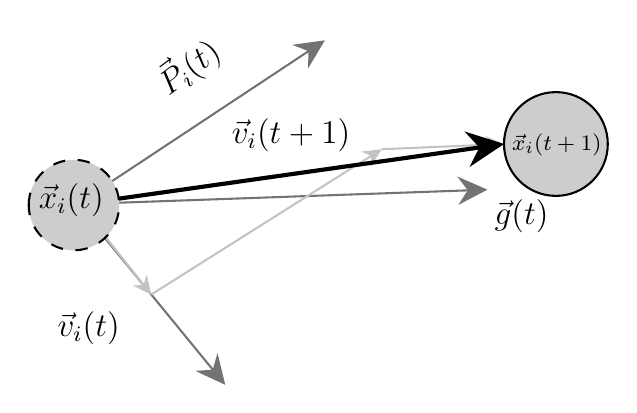
\begin{tikzpicture}[x=0.75pt,y=0.75pt,yscale=-1,xscale=1]
%uncomment if require: \path (0,300); %set diagram left start at 0, and has height of 300

%Straight Lines [id:da5958950638731724] 
\draw [color={rgb, 255:red, 115; green, 115; blue, 115 }  ,draw opacity=1 ]   (216,147) -- (410.61,140.11) ;
\draw [shift={(413.61,140)}, rotate = 177.97] [fill={rgb, 255:red, 115; green, 115; blue, 115 }  ,fill opacity=1 ][line width=0.08]  [draw opacity=0] (14.29,-6.86) -- (0,0) -- (14.29,6.86) -- (9.49,0) -- cycle    ;
%Straight Lines [id:da5519078451997654] 
\draw [color={rgb, 255:red, 115; green, 115; blue, 115 }  ,draw opacity=1 ]   (216,147) -- (332.81,69.71) ;
\draw [shift={(335.31,68.05)}, rotate = 146.51] [fill={rgb, 255:red, 115; green, 115; blue, 115 }  ,fill opacity=1 ][line width=0.08]  [draw opacity=0] (14.29,-6.86) -- (0,0) -- (14.29,6.86) -- (9.49,0) -- cycle    ;
%Straight Lines [id:da8436821411574322] 
\draw [color={rgb, 255:red, 115; green, 115; blue, 115 }  ,draw opacity=1 ]   (216,147) -- (285.41,231.73) ;
\draw [shift={(287.31,234.05)}, rotate = 230.68] [fill={rgb, 255:red, 115; green, 115; blue, 115 }  ,fill opacity=1 ][line width=0.08]  [draw opacity=0] (14.29,-6.86) -- (0,0) -- (14.29,6.86) -- (9.49,0) -- cycle    ;
%Straight Lines [id:da49229480545453086] 
\draw [color={rgb, 255:red, 197; green, 194; blue, 194 }  ,draw opacity=1 ]   (229,162) -- (249.79,188.18) ;
\draw [shift={(251.66,190.53)}, rotate = 231.54] [fill={rgb, 255:red, 197; green, 194; blue, 194 }  ,fill opacity=1 ][line width=0.08]  [draw opacity=0] (8.93,-4.29) -- (0,0) -- (8.93,4.29) -- (5.93,0) -- cycle    ;
%Straight Lines [id:da8102226735028486] 
\draw [color={rgb, 255:red, 197; green, 194; blue, 194 }  ,draw opacity=1 ]   (251.66,190.53) -- (360.12,122.13) ;
\draw [shift={(362.66,120.53)}, rotate = 147.76] [fill={rgb, 255:red, 197; green, 194; blue, 194 }  ,fill opacity=1 ][line width=0.08]  [draw opacity=0] (8.93,-4.29) -- (0,0) -- (8.93,4.29) -- (5.93,0) -- cycle    ;
%Straight Lines [id:da6537497146959208] 
\draw [color={rgb, 255:red, 197; green, 194; blue, 194 }  ,draw opacity=1 ]   (362.66,120.53) -- (418.61,118.13) ;
\draw [shift={(421.61,118)}, rotate = 177.55] [fill={rgb, 255:red, 197; green, 194; blue, 194 }  ,fill opacity=1 ][line width=0.08]  [draw opacity=0] (8.93,-4.29) -- (0,0) -- (8.93,4.29) -- (5.93,0) -- cycle    ;
%Shape: Circle [id:dp8574069381171916] 
\draw  [fill={rgb, 255:red, 205; green, 205; blue, 205 }  ,fill opacity=1 ] (421.61,118) .. controls (421.61,104.19) and (432.8,93) .. (446.61,93) .. controls (460.42,93) and (471.61,104.19) .. (471.61,118) .. controls (471.61,131.81) and (460.42,143) .. (446.61,143) .. controls (432.8,143) and (421.61,131.81) .. (421.61,118) -- cycle ;
%Straight Lines [id:da8931658978210233] 
\draw [line width=1.5]    (214.4,147.4) -- (417.65,118.56) ;
\draw [shift={(421.61,118)}, rotate = 171.92] [fill={rgb, 255:red, 0; green, 0; blue, 0 }  ][line width=0.08]  [draw opacity=0] (18.04,-8.67) -- (0,0) -- (18.04,8.67) -- (11.98,0) -- cycle    ;
%Shape: Circle [id:dp08907510762992255] 
\draw  [fill={rgb, 255:red, 205; green, 205; blue, 205 }  ,fill opacity=1 ][dash pattern={on 4.5pt off 4.5pt}] (192.61,147.4) .. controls (192.61,135.37) and (202.37,125.61) .. (214.4,125.61) .. controls (226.44,125.61) and (236.2,135.37) .. (236.2,147.4) .. controls (236.2,159.44) and (226.44,169.2) .. (214.4,169.2) .. controls (202.37,169.2) and (192.61,159.44) .. (192.61,147.4) -- cycle ;


% Text Node
\draw (289,104.4) node [anchor=north west][inner sep=0.75pt]  [font=\large]  {$\vec{v}_{i}( t+1)$};
% Text Node
\draw (424,111.4) node [anchor=north west][inner sep=0.75pt]  [font=\footnotesize]  {$\vec{x}_{i}( t+1)$};
% Text Node
\draw (415.61,143.4) node [anchor=north west][inner sep=0.75pt]  [font=\large]  {$\vec{g}( t)$};
% Text Node
\draw (196,135.4) node [anchor=north west][inner sep=0.75pt]  [font=\large]  {$\vec{x}_{i}( t)$};
% Text Node
\draw (248.64,82.49) node [anchor=north west][inner sep=0.75pt]  [font=\large,rotate=-323.22]  {$\vec{P_{i}}( t)$};
% Text Node
\draw (205,197.4) node [anchor=north west][inner sep=0.75pt]  [font=\large]  {$\vec{v}_{i}( t)$};


\end{tikzpicture}
